En este capítulo se describe la solución desarrollada en el proyecto alfredZ. El
objetivo del sistema es explorar autónomamente entornos interiores dinámicos
---con personas en movimiento--- construyendo un mapa de ocupación de alta
calidad. Para lograrlo se combinan técnicas de SLAM activo, detección semántica
de objetos dinámicos y planificación de rutas. En las secciones siguientes se
presentan los componentes del sistema, la lógica de selección de fronteras de
exploración y las estrategias implementadas para manejar la presencia de personas.

\section{Visión general del sistema}%
\label{sec:sol_overview}

El sistema alfredZ opera en un entorno de simulación construido con Gazebo,
donde un robot de tracción diferencial equipado con una cámara estéreo ZED
debe explorar un espacio desconocido que puede contener actores dinámicos
(personas) en movimiento. La plataforma de software utilizada es ROS~2 Humble,
sobre la cual se integran los siguientes componentes principales:

\begin{itemize}
    \item \textbf{RTAB-Map} (\textit{Real-Time Appearance-Based Mapping}):
          sistema de SLAM que construye el mapa de ocupación y estima la
          posición del robot a partir del flujo RGB-D de la cámara ZED\@.
    \item \textbf{Nav2}: pila de navegación de ROS~2 responsable de planificar
          rutas libres de obstáculos y ejecutar el movimiento del robot hacia
          las metas asignadas.
    \item \textbf{YOLOv8}: modelo de detección de objetos utilizado para
          identificar en tiempo real las personas presentes en el campo visual
          del robot.
    \item \textbf{DynamicMasker}: nodo propio que intercepta el flujo RGB-D
          antes de que llegue a RTAB-Map y enmascara las regiones
          correspondientes a personas detectadas, evitando que sean incorporadas
          al mapa estático.
    \item \textbf{SemanticNBVPlanner} (\textit{Next Best View Planner}): nodo
          central de toma de decisiones que detecta fronteras, calcula su
          utilidad y envía la meta de navegación a Nav2.
    \item \textbf{SemanticMetricsNode}: nodo que calcula y publica en tiempo
          real métricas de calidad del mapa y de detección de personas.
\end{itemize}

En la Figura~\ref{fig:arch_overview} se presenta un diagrama de los componentes
del sistema y el flujo de datos entre ellos.

\begin{figure}[h!]
    \centering
    \textcolor{red}{%
        [Imagen: diagrama de componentes y flujo de datos del sistema; mostrar el robot
        con la cámara ZED, la salida RGB-D llegando al DynamicMasker (que
        también recibe detecciones de YOLOv8), la salida enmascarada llegando
        a RTAB-Map, el mapa publicado en /map llegando al SemanticNBVPlanner
        (que también recibe la pose del robot de RTAB-Map y las detecciones de
        personas), el goal enviado a Nav2 y el cmd\_vel resultante al robot;
        SemanticMetricsNode se suscribe a /map y a /yolo/detections.]%
    }
    \caption{Diagrama de componentes y flujo de datos del sistema alfredZ.}%
    \label{fig:arch_overview}
\end{figure}

\section{Filtrado semántico de objetos dinámicos}%
\label{sec:sol_masker}

El principal desafío del mapeo en entornos dinámicos es que los sistemas de
SLAM convencionales asumen que el entorno es estático. Cuando
una persona se desplaza por el campo visual del robot, las lecturas de
profundidad correspondientes a su cuerpo se incorporan al mapa de ocupación
como obstáculos permanentes. Con el tiempo, esto produce \textit{ghost cells}:
celdas que el mapa marca como ocupadas pero que en realidad corresponden a
espacio libre donde la persona ya no se encuentra.

Para mitigar este problema se desarrolló el nodo \textbf{DynamicMasker}. Este
nodo se suscribe simultáneamente al flujo de imágenes de la cámara ZED (imagen
de color e imagen de profundidad) y a las detecciones publicadas por YOLOv8.
Cada vez que YOLOv8 detecta una persona, su bounding box se utiliza para
generar una máscara binaria sobre la imagen de profundidad: los píxeles
comprendidos dentro de la caja detectada se anulan (se les asigna profundidad
cero), de modo que RTAB-Map no recibe información de profundidad en esas
regiones y, por lo tanto, no las incorpora al mapa. La imagen de color se
enmascara de manera análoga.

Adicionalmente, el nodo mantiene un mapa de calor dinámico acumulado
(\textit{dynamic heatmap}) que registra las zonas del campo visual donde se
detectaron personas con mayor frecuencia, aplicando un factor de decaimiento
exponencial ($\alpha = 0{,}95$) para dar mayor peso a las detecciones recientes.
Este mapa de calor se publica como un \texttt{OccupancyGrid} y puede ser
utilizado por el planificador para tener noción de las zonas de mayor actividad
dinámica.

\section{Detección y agrupamiento de fronteras}%
\label{sec:sol_frontiers}

La exploración autónoma se basa en el concepto de \textbf{frontera}: el borde
entre el espacio ya conocido y el espacio aún desconocido del mapa. Moviéndose
hacia las fronteras, el robot amplía iterativamente la región mapeada hasta que
no quedan zonas por explorar.

\subsection{Representación del mapa de ocupación}

El mapa se recibe como un mensaje \texttt{nav\_msgs/OccupancyGrid}, que consiste
en una grilla regular de celdas con tres estados posibles:

\begin{itemize}
    \item $-1$: celda \textbf{desconocida} (no observada).
    \item $0$: celda \textbf{libre} (espacio navegable confirmado).
    \item $1$--$100$: celda \textbf{ocupada} (presencia de obstáculo,
          proporcional a la probabilidad de ocupación).
\end{itemize}

Cada celda se identifica por su índice $(fila, columna)$ en la grilla. La
posición en metros se obtiene a partir de la resolución y el origen del mapa.

\subsection{Definición e identificación de fronteras}

Una celda se considera \textbf{frontera} si cumple simultáneamente dos
condiciones: es libre ($valor = 0$) y al menos una de las ocho celdas que
forman su vecindad es desconocida ($valor = -1$). Esta vecindad de 8 celdas,
llamada vecindad~8 o conectividad~8, incluye las celdas adyacentes en las
cuatro direcciones cardinales y las cuatro diagonales.

En la Figura~\ref{fig:frontier_def} se ilustra esta definición con un ejemplo.

\begin{figure}[h!]
    \centering
    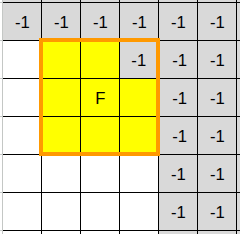
\includegraphics[width=0.52\textwidth]{figures/methodology/fig_frontier_def.png}
    \medskip
    \begin{minipage}{0.80\textwidth}
        \footnotesize
        \centering
        \begin{tabular}{@{}p{0.35\textwidth}p{0.58\textwidth}@{}}
            \textbf{Blanco} & Celda libre (valor $0$). \\
            \textbf{Gris con ``$-1$''} & Celda desconocida (no observada). \\
            \textbf{F} & Celda \emph{frontera}: libre con al menos un vecino
            desconocido en su vecindad~8. \\
            \textbf{Borde naranja} ($3\times 3$) & Vecindad~8 (conectividad de
            Moore) centrada en la celda \textbf{F}. \\
            \textbf{Sombreado amarillo} & Celdas incluidas en la vecindad usada en
            el ejemplo. \\
        \end{tabular}
    \end{minipage}
    \caption{Definición de frontera: celda libre con al menos una celda
    desconocida en su vecindad~8 (recuadro 3$\times$3).}%
    \label{fig:frontier_def}
\end{figure}

La identificación se implementa mediante operaciones matriciales con la
biblioteca SciPy. Primero se obtiene la máscara de celdas desconocidas y
se la dilata con una estructura de conectividad~8; el resultado representa
todas las celdas adyacentes a zonas desconocidas. La intersección de esta
máscara dilatada con la máscara de celdas libres produce el conjunto de celdas
frontera, de forma equivalente a la definición anterior pero de manera
vectorizada y eficiente.

\subsection{Agrupamiento en clusters}

Las celdas frontera identificadas no se tratan de forma individual sino que
se agrupan en \textbf{clusters} mediante un algoritmo de etiquetado de
componentes conexas con conectividad~8. Cada cluster representa una zona
continua de frontera y se caracteriza por tres elementos:

\begin{itemize}
    \item \textbf{Representante}: la celda del cluster más cercana a su
          centroide geométrico, utilizada como objetivo de navegación.
    \item \textbf{Celdas}: el conjunto completo de celdas $(fila, columna)$
          que conforman el cluster.
    \item \textbf{Ganancia de información estática} ($IG_{est\acute{a}tica}$):
          el número de celdas desconocidas en la vecindad del cluster,
          que estima cuánta información nueva se obtendría al visitarlo.
\end{itemize}

Los clusters con menos de un número mínimo configurable de celdas
(\texttt{min\_cluster\_cells}) son descartados para evitar fronteras espurias.

\subsection{Pre-filtrado por ganancia de información}

Dado que calcular el costo de trayecto hasta cada frontera mediante Nav2 es
una operación costosa, se aplica un \textbf{pre-filtrado} antes de evaluar la
función de utilidad completa: se ordenan los clusters por $IG_{est\acute{a}tica}$
de mayor a menor y se retienen solo los \texttt{max\_frontiers\_to\_evaluate}
más prometedores. Los costos de trayecto se calculan en paralelo solo para
estas fronteras preseleccionadas.

\section{Función de utilidad para selección de Next Best View}%
\label{sec:sol_utility}

Para decidir cuál frontera visitar en cada iteración, se define una función de
utilidad $U(v)$ que balancea tres factores: la cantidad de información nueva que
se obtendría al visitar la frontera, el costo de llegar a ella y la presencia de
personas en su entorno. La frontera seleccionada es aquella que maximiza $U(v)$:

\begin{equation}
    U(v) = IG_{est\acute{a}tica}(v) - \lambda \cdot Din\acute{a}mica(v) - \mu \cdot Costo_{trayecto}(v)
    \label{eq:utility}
\end{equation}

donde:

\begin{itemize}
    \item $IG_{est\acute{a}tica}(v)$: número de celdas desconocidas en la
          vecindad del cluster $v$. Cuanto mayor, más información nueva se
          espera obtener al visitar esa zona.
    \item $Din\acute{a}mica(v)$: estimación de la interferencia de personas
          en el entorno de $v$. El cálculo concreto depende de la estrategia
          seleccionada (Sección~\ref{sec:sol_strategies}).
    \item $Costo_{trayecto}(v)$: longitud en metros de la ruta planificada
          por Nav2 desde la posición actual del robot hasta el representante
          de $v$. Se calcula en paralelo para todas las fronteras
          preseleccionadas.
    \item $\lambda$: parámetro de penalización sobre la interferencia dinámica.
          Un valor $\lambda = 0$ equivale a ignorar completamente la presencia
          de personas.
    \item $\mu$: parámetro de penalización sobre el costo de trayecto.
          Valores más altos favorecen fronteras más cercanas al robot.
\end{itemize}

En la Figura~\ref{fig:frontier_ig} se ilustra cómo varía $IG_{est\acute{a}tica}$
según la configuración de celdas desconocidas alrededor de una frontera.

\begin{figure}[h!]
    \centering
    \begin{subfigure}{0.31\textwidth}
        \centering
        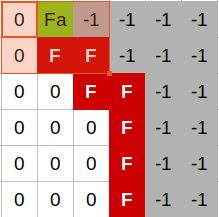
\includegraphics[width=\linewidth]{figures/methodology/frontier_ig_1.png}
        \caption{$IG_{est\acute{a}tica}=1$}
    \end{subfigure}\hfill
    \begin{subfigure}{0.31\textwidth}
        \centering
        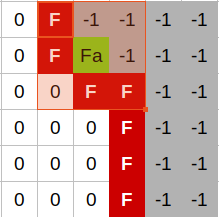
\includegraphics[width=\linewidth]{figures/methodology/frontier_ig_3.png}
        \caption{$IG_{est\acute{a}tica}=3$}
    \end{subfigure}\hfill
    \begin{subfigure}{0.31\textwidth}
        \centering
        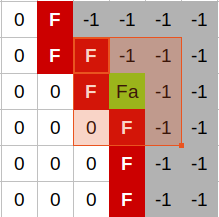
\includegraphics[width=\linewidth]{figures/methodology/frontier_ig_4.png}
        \caption{$IG_{est\acute{a}tica}=4$}
    \end{subfigure}
    \caption{Ejemplos de $IG_{est\acute{a}tica}$ para distintas configuraciones
    de celdas desconocidas alrededor de una frontera~$F_a$.}%
    \label{fig:frontier_ig}
\end{figure}

\section{Estrategias de exploración}%
\label{sec:sol_strategies}

Se implementaron cuatro modos de operación del planificador que difieren en
la forma en que se calcula el término $Din\acute{a}mica(v)$ de la función de
utilidad. Tres de ellos constituyen las estrategias propias de alfredZ (E1, E2
y E3) y uno actúa como \textit{baseline} de referencia (Greedy).

\subsection{Greedy (baseline)}

En el modo Greedy el planificador selecciona siempre la frontera más cercana
al robot según la distancia euclídea, sin considerar el costo de trayecto
planificado ni la presencia de personas ($\lambda = 0$, $\mu = 0$). Esta
estrategia es el punto de comparación mínimo: explora el mapa de forma simple
y rápida pero es completamente ciega a los agentes dinámicos.

\subsection{Estrategia E1: Frontera}

La Estrategia~E1 define $Din\acute{a}mica(v)$ como la cantidad de personas
detectadas dentro de un radio $r$ alrededor del representante de la frontera $v$:

\begin{equation}
    Din\acute{a}mica_{E1}(v) = \left|\left\{p \in P \;\middle|\; \|pos(p) - centro(v)\| \leq r\right\}\right|
    \label{eq:e1}
\end{equation}

donde $P$ es el conjunto de personas detectadas y $pos(p)$ es la posición
estimada de la persona $p$ en el plano del mapa. Cuantas más personas haya
cerca de una frontera, mayor es su costo dinámico y menor su utilidad. De esta
forma el planificador tiende a evitar fronteras en zonas concurridas en favor
de aquellas en zonas libres de personas.

\subsection{Estrategia E2: Ruta planificada}

La Estrategia~E2 amplía el criterio de~E1 considerando no solo la proximidad a
la frontera destino sino la presencia de personas a lo largo de todo el trayecto
planificado por Nav2 hasta ella:

\begin{equation}
    Din\acute{a}mica_{E2}(v) = \left|\left\{p \in P \;\middle|\; \exists\, q \in Ruta(v) : \|pos(p) - q\| \leq r\right\}\right|
    \label{eq:e2}
\end{equation}

donde $Ruta(v)$ es el conjunto de puntos de la ruta planificada hasta $v$.
El planificador penaliza las fronteras cuyo camino de acceso está bloqueado o
concurrido, priorizando rutas que puedan recorrerse con menor interferencia.

\subsection{Estrategia E3: Predictiva}

La Estrategia~E3 incorpora un modelo de predicción de movimiento para anticipar
la posición futura de las personas. A partir del historial de posiciones de cada
actor, se estima su velocidad promedio y se predice dónde estará al momento en
que el robot llegue a la frontera (en un tiempo de viaje $t$ segundos):

\begin{equation}
    \hat{pos}(p, t) = pos(p) + \bar{v}(p) \cdot t
    \label{eq:pred}
\end{equation}

El costo dinámico se calcula entonces como en E2 pero usando las posiciones
predichas $\hat{pos}(p, t)$ en lugar de las posiciones actuales. Esta estrategia
permite al planificador evitar proactivamente rutas que, aunque libres en el
momento de la decisión, se estima que estarán bloqueadas cuando el robot las
recorra.

En la Figura~\ref{fig:strategies} se presenta una comparación conceptual de
las tres estrategias.

\begin{figure}[h!]
    \centering
    \begin{subfigure}{0.31\textwidth}
        \centering
        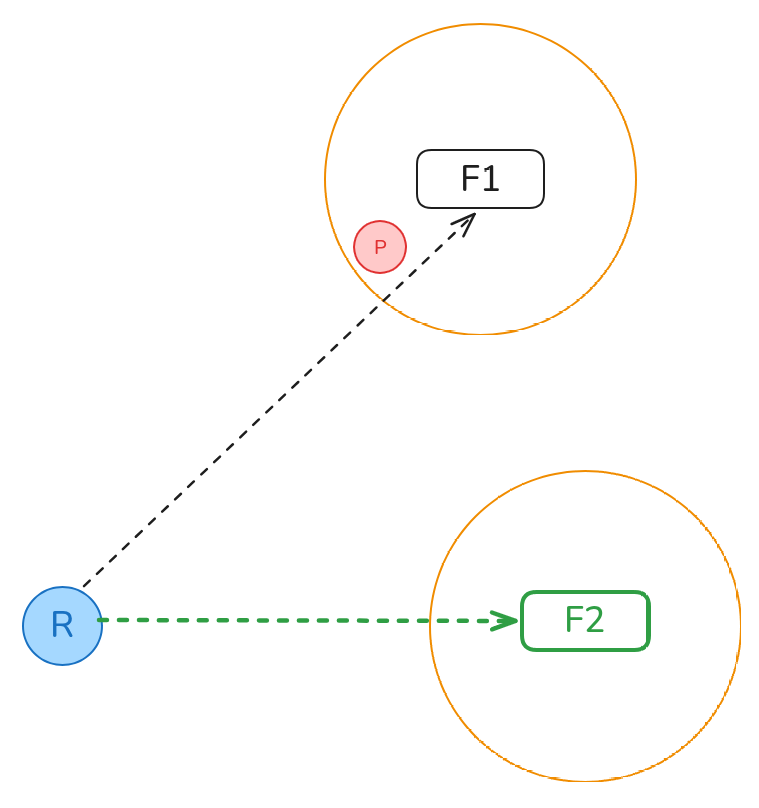
\includegraphics[width=\linewidth]{figures/methodology/strategies_e1.png}
        \caption{E1 (Frontera): se penaliza la proximidad de personas a la frontera.}
    \end{subfigure}\hfill
    \begin{subfigure}{0.31\textwidth}
        \centering
        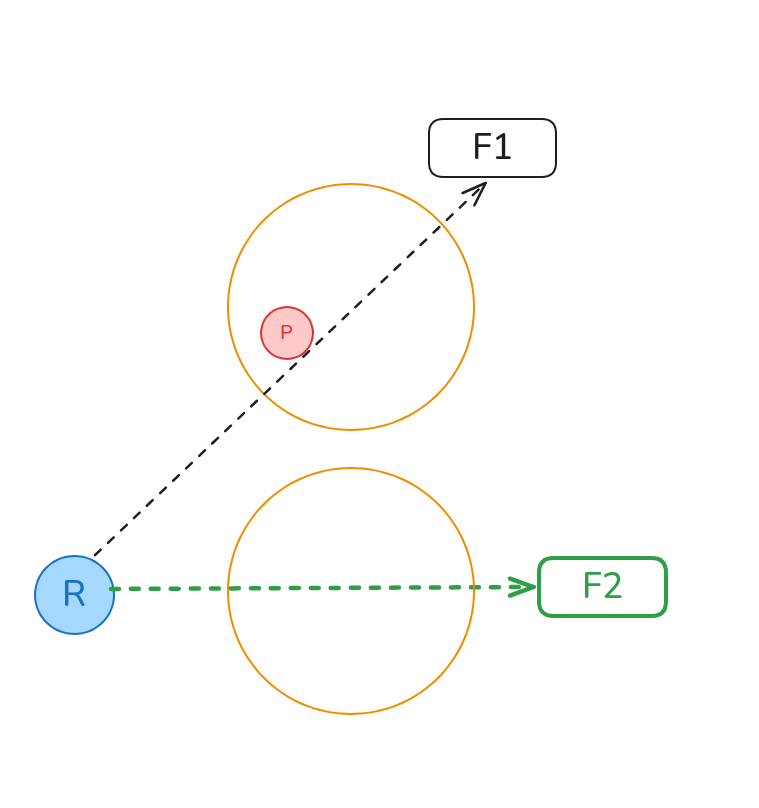
\includegraphics[width=\linewidth]{figures/methodology/strategies_e2.png}
        \caption{E2 (Ruta planificada): se penaliza la interferencia sobre la ruta.}
    \end{subfigure}\hfill
    \begin{subfigure}{0.31\textwidth}
        \centering
        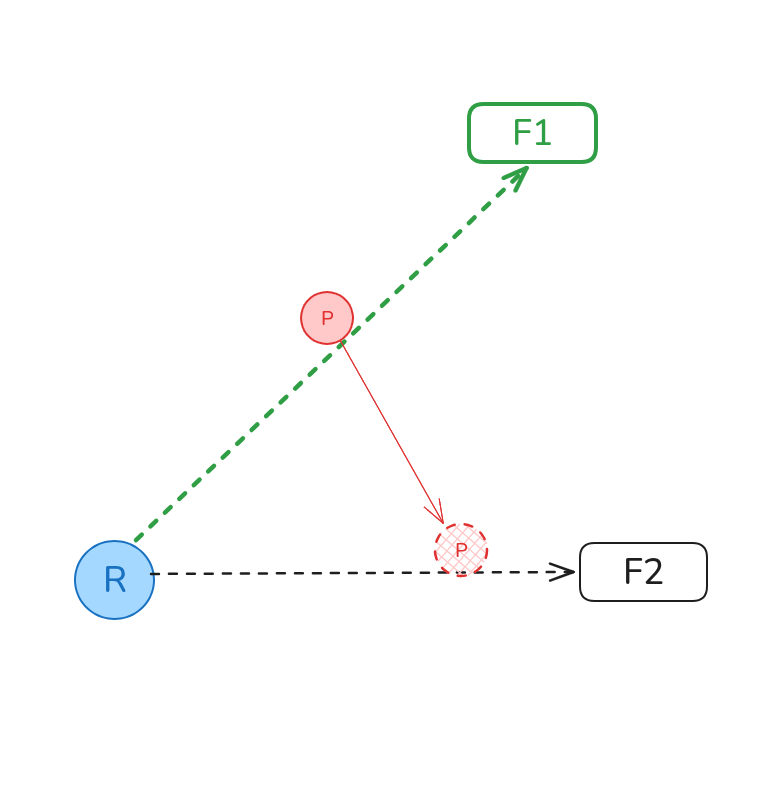
\includegraphics[width=\linewidth]{figures/methodology/strategies_e3.png}
        \caption{E3 (Predictiva): se penaliza la interferencia esperada en el futuro.}
    \end{subfigure}
    \par\vspace{0.6em}
    \begin{minipage}{0.95\textwidth}
        \footnotesize
        \textit{Convenciones:} \textbf{R} = robot, \textbf{P} = persona detectada,
        \textbf{$F_1$/$F_2$} = fronteras candidatas, \textbf{flecha verde} =
        ruta/fontera seleccionada, \textbf{línea negra punteada} = alternativa no
        seleccionada, \textbf{círculo naranja} = zona de evaluación local, y en E3 la
        \textbf{persona rayada} representa la posición predicha.
    \end{minipage}
    \caption{Comparación conceptual de las estrategias E1 (Frontera), E2 (Ruta
    planificada) y E3 (Predictiva). La frontera seleccionada en cada caso se
    indica con un recuadro verde.}%
    \label{fig:strategies}
\end{figure}

\section{Métricas de evaluación semántica}%
\label{sec:sol_metrics}

Para cuantificar el impacto de los agentes dinámicos en la calidad del mapa se
diseñaron métricas específicas que se calculan y publican en tiempo real por el
nodo SemanticMetricsNode.

\subsection{Celdas fantasma}

Las \textbf{celdas fantasma} (\textit{ghost cells}) son celdas que el mapa
registra como ocupadas en el momento actual pero que en observaciones recientes
estaban libres. Formalmente, dado el mapa actual $M_t$ y los mapas de los
últimos $k$ instantes $\{M_{t-k}, \ldots, M_{t-1}\}$, el número de celdas
fantasma se calcula como:

\begin{equation}
    GC(t) = \sum_{i=1}^{k} \left|\left\{(r,c) \;\middle|\; M_t(r,c) > 50 \;\wedge\; M_{t-i}(r,c) < 50\right\}\right|
    \label{eq:ghost}
\end{equation}

Un valor elevado de $GC$ indica que el mapa contiene muchas ocupaciones
transitorias causadas por personas en movimiento. A medida que el sistema de
filtrado semántico funciona correctamente, el valor de $GC$ debería mantenerse
bajo incluso en escenarios con muchos actores.

\subsection{Entropía del mapa}

La \textbf{entropía del mapa} cuantifica la incertidumbre global del mapa de
ocupación. Un mapa de alta calidad debería presentar celdas con valores
claramente definidos (libre u ocupado), mientras que un mapa degradado por
agentes dinámicos tendrá más celdas con valores intermedios o inconsistentes.
La entropía se calcula sobre las celdas conocidas (valor $\geq 0$) del mapa:

\begin{equation}
    H = -\sum_{(r,c)\,:\,M(r,c) \geq 0} p_{r,c} \cdot \log_2(p_{r,c})
    \label{eq:entropy}
\end{equation}

donde $p_{r,c} = M(r,c) / 100$ es la probabilidad de ocupación de la celda.
Valores de entropía más altos indican mayor incertidumbre en el mapa.

\subsection{Métricas de detección de personas}

Complementariamente se registran métricas sobre la actividad de los actores
dinámicos durante cada experimento:

\begin{itemize}
    \item \textbf{Total de frames procesados}: número de frames en los que
          YOLOv8 realizó al menos una detección.
    \item \textbf{Promedio de personas por frame}: promedio de personas
          detectadas en cada frame procesado, indicador de la densidad de
          actividad dinámica.
    \item \textbf{Máximo de personas detectadas simultáneamente}: número máximo
          de personas presentes en un mismo frame, útil para caracterizar los
          picos de concurrencia.
\end{itemize}
